\section{Proof of Proposition~\ref{prop:consistency}}
\label{app:proofs}

We write $n=2N$ for the number of units and index them by $a=(i,\tau)$, $\tau\in\{t_0,t\}$. Throughout, $\|\cdot\|$ is the Euclidean norm and $W$ is the orthogonal matrix of \eqref{eq:conc}; since the scan statistic \eqref{eq:TS} and the candidate family of Section~\ref{sec:scan} are invariant to a common orthogonal transformation of the displacements, we may take $W=I$ without loss of generality.

\paragraph{Step 1: displacements concentrate.}
By \citet[Theorem~1]{pkps2026} applied to the $n$ units, with probability at least $1-\eta$,
$\max_a\|\hat\psi_a-\psi_a\|\le\varepsilon_m$, so for every agent
\begin{equation}
\label{eq:disp-conc}
\|\hat\Delta_i-\Delta_i\| \;\le\; \|\hat\psi_{(i,t)}-\psi_{(i,t)}\| + \|\hat\psi_{(i,t_0)}-\psi_{(i,t_0)}\| \;\le\; 2\varepsilon_m .
\end{equation}
Under \eqref{eq:model} the population displacements are $\Delta_i = c + \delta v\,\ind\{i\in S\}$. Let $\rho=|S|/N<1/2$. The coordinate-wise median of $\{\hat\Delta_i\}$ lies within $2\varepsilon_m$ of the coordinate-wise median of $\{\Delta_i\}$, which equals $c$ because the majority of agents have $\Delta_i=c$; hence the centered estimates satisfy
\begin{equation}
\label{eq:centered}
\|\tilde\Delta_i - \delta v\,\ind\{i\in S\}\| \;\le\; 4\varepsilon_m \qquad\text{for all } i .
\end{equation}

\paragraph{Step 2: the family contains $S$.}
By \eqref{eq:centered}, the centered estimates of agents in $S$ lie in a ball of radius $4\varepsilon_m$ about $\delta v$ and those outside $S$ in a ball of the same radius about $0$. If $\delta>16\varepsilon_m$ the two balls are separated by more than $8\varepsilon_m$, which exceeds the diameter of each. Any $2$-means solution with the optimal objective must then place the two balls in different clusters: a partition that splits a ball has within-cluster sum of squares at least $(\delta-8\varepsilon_m)^2/4$ per split point, while the ball partition has objective at most $N(4\varepsilon_m)^2$, and the former exceeds the latter once $\delta/\varepsilon_m$ is large enough. (The same argument applies to the whitened displacements since whitening with the trimmed covariance, which concentrates on the majority ball, changes distances by at most a bounded factor.) Hence $S$ is one of the two clusters at $k=2$. Independently, the leading direction $w$ of the whitened displacements is within a small angle of $v$ by the Davis--Kahan theorem, and ordering the agents by $|w^\top\tilde\Delta_i|$ places the $|S|$ agents of $S$ first; so $S$ is also the top-$|S|$ nested set. Either way $S\in\Sfam$ on the event of \eqref{eq:disp-conc}.

\paragraph{Step 3: the statistic separates.}
On the same event, $T(S)\ge|S|(\delta-4\varepsilon_m)^2/\lambda_{\max}(\hat\Sigma)$ and, for any $S'\in\Sfam$ with $S'\ne S$, either $S'\subsetneq S$ (so $T(S')\le|S'|(\delta+4\varepsilon_m)^2/\lambda_{\min}(\hat\Sigma)<T(S)$ once $\delta/\varepsilon_m$ is large, because $|S'|<|S|$) or $S'$ contains agents outside $S$, in which case $\|\bar\Delta_{S'}\|\le\frac{|S'\cap S|}{|S'|}\delta+4\varepsilon_m$ and $T(S')\le\frac{|S'\cap S|^2}{|S'|}(\delta+4\varepsilon_m)^2/\lambda_{\min}<T(S)$ for the same reason since $|S'\cap S|^2/|S'|<|S|$ strictly. The trimmed covariance has eigenvalues of the order of the displacement noise variance $\sigma^2$, which is bounded above and below on the event of \eqref{eq:disp-conc} under the sub-Gaussian assumption. Hence $\hat S=\argmax_{S'\in\Sfam}T(S')=S$, and $\Lambda\ge c\,|S|\delta^2/\sigma^2$ after the size standardization of Section~\ref{sec:scan}, whose per-size null moments are bounded.

\paragraph{Step 4: the permutation null is bounded.}
Under each permutation, every agent's (query, response) pairs are reassigned across the two time points, so the permuted displacements satisfy \eqref{eq:disp-conc} with $\delta=0$ (the permuted units have the mixture conditional distribution at both time points). Every $T(S')$ in the permuted family is then at most $|S'|(4\varepsilon_m)^2/\lambda_{\min}$, and after size standardization the permuted scan statistics are bounded by a constant depending on the family size $O(KN)$ and the sub-Gaussian scale. Since $\Lambda$ diverges as $|S|\delta^2/\sigma^2\to\infty$ while the permutation statistics remain bounded, the $p$-value tends to zero on the event of \eqref{eq:disp-conc}, which has probability at least $1-\eta$ for any fixed $\eta$. Taking $\eta\to 0$ along $m\to\infty$ completes the proof. \qed

\begin{remark}
The argument uses the concentration bound only through \eqref{eq:disp-conc}, so any representation with a comparable guarantee may be substituted for PKPS; and it uses the family only through the fact that $S$ is a 2-means cluster and a nested set once the balls separate, so any family that contains the clusters of a consistent clustering suffices. The constants are loose; the simulations of Section~\ref{sec:sims} show that separation is in fact reached well before $\delta/\varepsilon_m$ is large.
\end{remark}

\section{Additional simulation results}
\label{app:sims}

\begin{figure}[h]
  \centering
  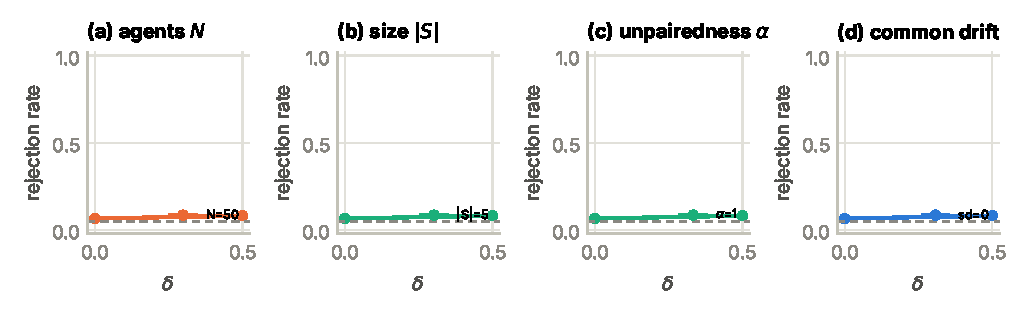
\includegraphics[width=\textwidth]{figures/sim_detection_appendix.pdf}
  \caption{Experiment 1 (detection), remaining factors. Rejection rate versus $\delta$ by (a) number of agents $N$ with $|S|=5$ fixed, (b) subnetwork size $|S|$, (c) topic concentration $\alpha$ (small is unpaired), (d) common drift. \todo{to be rendered from the full run}}
  \label{fig:sim-detect-app}
\end{figure}

\todo{Per-cell Type~I table; conditional-on-rejection membership metrics; sensitivity to $d$, bandwidth, and family size $K$.}
